\documentclass[12pt,a4paper]{article}
\usepackage[utf8]{inputenc}
\usepackage[margin=1in]{geometry}
\usepackage{graphicx}
\usepackage{amsmath}
\usepackage{amsfonts}
\usepackage{enumerate}
\usepackage{listings}

\lstset{
    basicstyle=\ttfamily\small, % Font style and size
    numbers=left,               % Line numbers on the left
    numberstyle=\tiny,          % Line number style
    frame=single,               % Frame around the code
    breaklines=true,            % Allow line breaking
    captionpos=b                % Caption position (b for below)
}

% Title and Author
\title{TMA4162 Computational algebra, Project 2}
\author{Andreas Moe}
\date{\today}

\begin{document}

\maketitle

\section*{Task 1, Theory}
\begin{enumerate}[a)]
    \item 
\end{enumerate}

\section*{Task 2, Practice}

\begin{enumerate}[a)]
    \item 
\end{enumerate}

\begin{figure}[htbp]
    \centering
    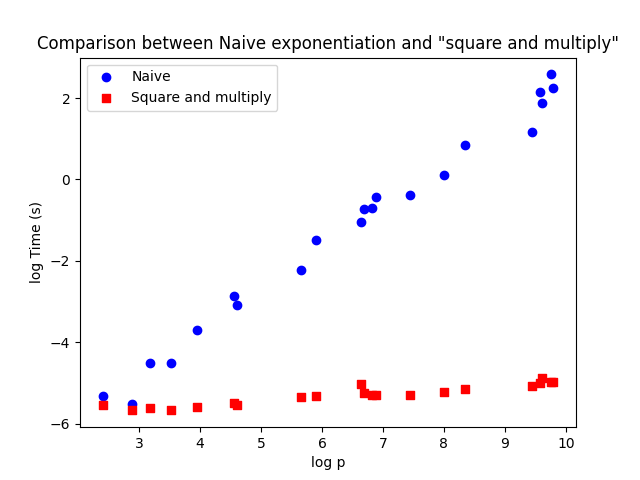
\includegraphics[width=\linewidth]{plot_2025-01-24 14-39-00_0.png}
    \caption{Measurements}
    \label{figure1}
\end{figure}
\newpage
\begin{appendix}
\section*{Appendix}
    Code is available at https://github.com/andrmoe/ComputationalAlgebra
    \lstinputlisting[language=Python, caption={prime.py}, label={lst:python_code}]{prime.py}
\end{appendix}

\end{document}
